\section{Shutdown}

\begin{frame}
\Huge{\centerline{Shutdown}}
\end{frame}

\begin{frame}
After we the participants are done communicating the protocol must shut down.
\vfill
During this phase the participants will

  \begin{itemize}
    \item Determine that there are no more messages in-flight.
    \item Verify the consistency of their transcripts.
    \item Destroy the session and delete any ephemeral secrets.
  \end{itemize}
\end{frame}


\begin{frame}
To establish that there is a consensus over the set of the messages, each participant $X$ hashes his \emph{sent} list (ordered lexicographically), producing the hash $h_x$ and broadcasts the tuple $\langle "shutdown", h_x \rangle$.\\[0.5cm]

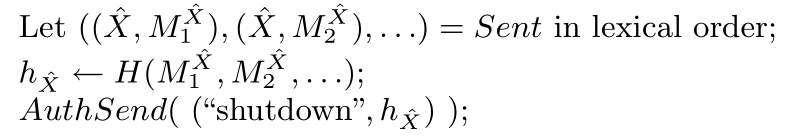
\includegraphics[scale=0.4]{Figures/sent_hash.png}
\end{frame}

\begin{frame}
After that he will patiently wait to receive the shutdown message from all  other participants.\\[0.5cm]

When he receives a shutdown message from user $Y$ he shall hash on his own $Y$'s \emph{received} list  and mark that he is no longer waiting messages from user $Y$.\\[0.5cm]

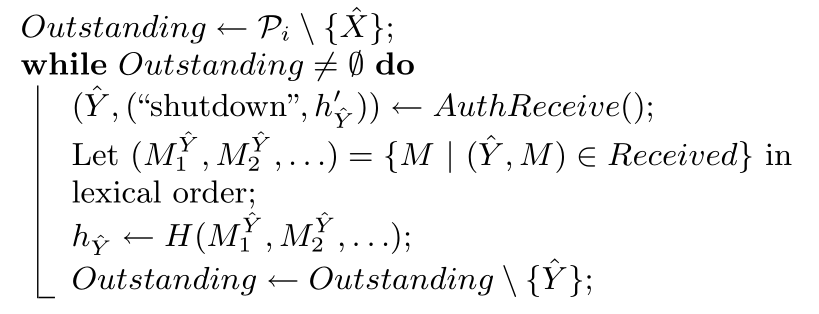
\includegraphics[scale=0.4]{Figures/received_hashes.png}
\end{frame}

\begin{frame}
After he has received the shutdown messages from all users he will hash his \emph{sent} hash with all the received hashes together, producing a digest $h$ of the whole chat, and broadcasts the tuple $\langle "digest", h \rangle$.\\[0.5cm]

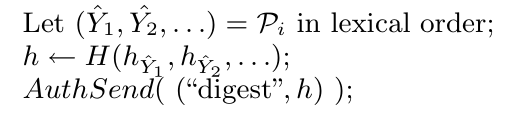
\includegraphics[scale=0.4]{Figures/chat_digest.png}
\end{frame}

\begin{frame}
He will again wait to receive the digest messages from all other users and compare the received digests with the one he produced earlier in order to determine if a consensus is reached.\\[0.5cm]

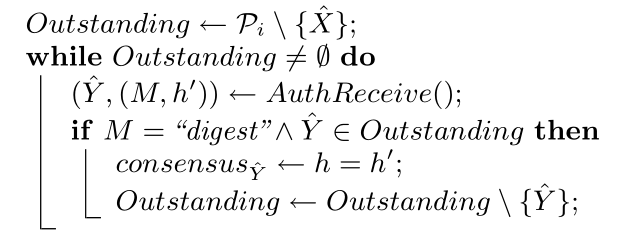
\includegraphics[scale=0.4]{Figures/determine_consensus.png}
\end{frame}

\begin{frame}
After that he informs the other users that he does not intend to send any messages, and waits to receive such confirmations from the rest of the users.\\[0.5cm]

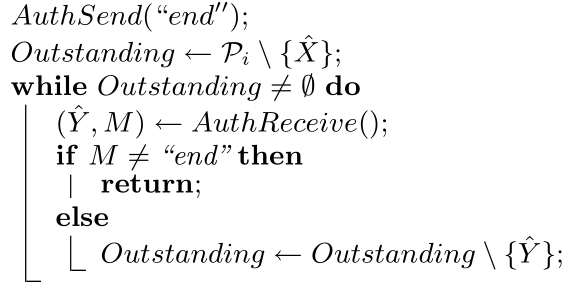
\includegraphics[scale=0.4]{Figures/no_listen_verify.png}\\[1cm]

And finally he broadcasts his signing key.
\end{frame}
